\chapter{Resultados} \label{chapter:III}
\section{Scrum en la pr\'{a}ctica (1ra Iteraci\'{o}n)}
\begin{spacing}{1.5}
	\subsection{\textit{Produc BackLog}}
	Se definieron 15 historias como l\'{i}nea base (ver figura \ref{figure:chaperIII_1}) que trataron temas de compatibilidad, escalabilidad, integraci\'{o}n y nuevas funcionalidades.
	\begin{figure}[H]
		\centering
		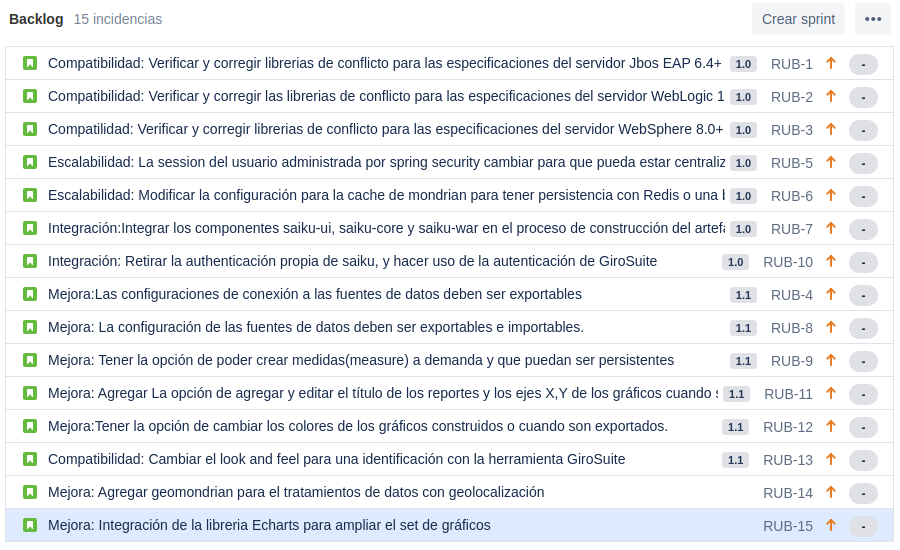
\includegraphics[width=1 \textwidth]{scrum_3_1}
		\caption {\centering \small{Product BackLog}} \label{figure:chaperIII_1}
		\small {Fuente: \'{A}rea de desarrollo de Tesla Technologies S.A.C, 2018}
	\end{figure}
	\clearpage
	\textbf{Compromiso: Objetivo del Producto}\\
	``Integrar las funcionalidades core de Saiku Analytics y que su compatibilidad al 100\% en la infraestructura de los clientes donde esta instalda la herramienta GiroSuite''.\\
	En la primera interaci\'{o}n se tomaron 7 historias, como se muestra en la tabla. 
	\begin{table}[bth]\centering\small
	\begin{tabular}[H]{m{0.1\linewidth}m{0.1\linewidth}|m{0.6\linewidth} m{0.12\linewidth}}
			\hline
			\rowcolor[HTML]{CBCEFB} 
			\textbf{Tipo} & \textbf{Clave} &\textbf{Resumen} &\textbf{Estado}\\
			\hline
			Historia &RUB-10 &Integración: Retirar la authenticación propia de saiku, y hacer uso de la autenticación de GiroSuite &Tareas por hacer.\\
			\hline
			Historia &RUB-7 &Integración:Integrar los componentes saiku-ui, saiku-core y saiku-war en el proceso de construcción del artefacto de GiroSuite. &Tareas por hacer\\
			\hline
			Historia &RUB-6 &Escalabilidad: Modificar la configuración para la cache de mondrian para tener persistencia con Redis o una base de datos relacional. &Tareas por hacer\\
			\hline
			Historia &RUB-5 &Escalabilidad: La session del usuario administrada por spring security cambiar para que pueda estar centralizada en la base de datos. &Tareas por hacer\\
			\hline
			Historia &RUB-3 &Compatilidad: Verificar y corregir librerias de conflicto para las especificaciones del servidor WebSphere 8.0+ y los archivos ibm-web-bnd.xml, ibm-web-ext.xml, deployment.xml y build.properties &Tareas por hacer\\
			\hline
			Historia &RUB-2 &Compatibilidad: Verificar y corregir las librerias de conflicto para las especificaciones del servidor WebLogic 12c + y los archivos weblogic.xml y build.properties &Tareas por hacer\\
			\hline
			Historia &RUB-1 &Compatibilidad: Verificar y corregir librerias de conflicto para las especificaciones del servidor Jbos EAP 6.4+ y loss archivos jboss-deployment-structure.xml, application.xml y build.properties. &Tareas por hacer\\
			\hline
		\end{tabular}
	\caption{Historias de la primera iteraci\'{o}n}
	\small {Fuente: \'{A}rea de desarrollo de Tesla Technologies S.A.C, 2018}
	\label{table:III_1}
	\end{table}

	\subsection{\textit{Sprint Planning}}
	\subsection{\textit{Sprint BackLog}}
	\subsection{\textit{Daily Scrum} (Durante 20 d\'{i}as)}
	\subsection{\textit{Sprint Review}}
	\subsection{\textit{Sprint Retrospective}}
	
	\subsection{\textit{Increment}}
\end{spacing}